\chapter{Runge-Kutta Method}
The \addtoindex{Runge-Kutta method} (RK) method is closely related to the Taylor series expansions but no differentiation of $f$ is necessary.\\
All RK methods will be written in the form
\begin{equation}
\label{RK A}
w_{n+1} =w_n +hF(t,w,h;f), \ \ \ n\geq 0.
\end{equation}
The truncation error for (\ref{RK A}) is defined by
\[
T_{n}(y) =y(t_{n+1})-y(t_n) -hF(t_n,y(t_n),h;f) 
\]
where the error is written as $\tau_n(y)$ 
\[ T_n=h\tau_n(y).\]
Rearranging we get
\[
y(t_{n+1})=y(t_n) -h F(t_n,y(t_n),h;f) +
h\tau_n(y).\]


\begin{theorem} \label{RK_Theorem}
Suppose f(t,y) and all its partial derivatives of order less than or equal to
n+1 are continuous on $D=\{(t,y)|a\leq t \leq b, c \leq y \leq d \}$ and let 
$(t_0,y_0)\in D$ for every $(t,y)\in D$, $\exists \ \ \xi \in (t,t_0)$ and $\mu \in (y,y_0)$ with
\[f(t,y) = P_n(t,y) + R_n(t,y) \]
where
\begin{eqnarray*}
 P_n(t,y) &=& f(t_0,y_0)+\left[(t-t_0)\frac{\partial f}{\partial t}(t_0,y_0)+(y-y_0)\frac{\partial f}{\partial y}(t_0,y_0) \right]\\
& & + \left[\frac{(t-t_0)^2}{2}\frac{\partial^2 f}{\partial t^2}(t_0,y_0)+(y-y_0)(t-t_0)\frac{\partial^2 f}{\partial y\partial t}(t_0,y_0)\right. \\
& & +\left. \frac{(y-y_0)^2}{2}\frac{\partial^2 f}{\partial y^2}(t_0,y_0) \right]\\
& & +...+\\
& & + \left[\frac{1}{n!}\sum_{j=0}^n\left(\begin{array}{c}n \\ j \end{array}\right)(t-t_0)^{n-j}(y-y_0)^j\frac{\partial^n f}{\partial y^j\partial t^{n-j}}(t_0,y_0)  \right]
\end{eqnarray*}
and
\begin{eqnarray*}\begin{aligned}R_n(t,y) = \\\left[\frac{1}{(n+1)!}\sum_{j=0}^{n+1}\left(\begin{array}{c}n+1 \\ j \end{array}\right)(t-t_0)^{n+1-j}(y-y_0)^j\frac{\partial^{n+1} f}{\partial y^j\partial t^{n+1-j}}(\xi,\mu)  \right]\end{aligned}
\end{eqnarray*}
\end{theorem}
\section{Derivation of Second Order Runge-Kutta}
Consider the explicit one-step method\\
\begin{equation}
\frac{w_{i+1}-w_i}{h}=F(f,t_i,w_i,h)
\end{equation}
with
\begin{equation}
F(f,t,y,h)=a_0k_1+a_1k_2,
\end{equation}
\begin{equation}
F(f,t,y,h)=a_0f(t,y)+a_1f(t+\alpha_1,y+\beta_1),
\end{equation}
where $a_0+a_1=1.$\\
\textbf{There is a free parameter in the derivation of the Runge-Kutta method for this reason $a_0$ must be choosen}

Deriving the second order \addtoindex{Runge-Kutta method} by using Theorem \ref{RK_Theorem} to determine values for values  $a_1,\alpha_1$ and $\beta_1$ with the property that $a_1f(t+\alpha_1,y+\beta_1)$ approximates the second order Taylor
\[f(t,y)+\frac{h}{2}f^{'}(t,y) \]
with error no greater than than $O(h^2)$, the local truncation error for
the Taylor method of order two.\\
Using
\[f^{'}(t,y)=\frac{\partial f}{\partial t}(y,t)+\frac{\partial f}{\partial y}(t,y).y^{'}(t), \]
the second order Taylor can be re-written as
\begin{equation}
\label{RKA}
f(t,y)+\frac{h}{2}\frac{\partial f}{\partial t}(y,t)+\frac{h}{2}\frac{\partial f}{\partial y}(t,y).f(t,y).
\end{equation}
Expanding $a_1f(t+\alpha_1,y+\beta_1)$ in its Taylor polynomial of degree one about
$(t,y)$ gives
\begin{equation}
\label{RKB}
a_1f(t+\alpha_1,y+\beta_1)= a_1 f(t,y) +a_1 \alpha_1 \frac{\partial f}{\partial t}(t,y)+a_1 \beta_1\frac{\partial f}{\partial y}+a_1R_1(t+\alpha_1,y+\beta_1)
\end{equation}
where
\[ R_1(t+\alpha_1,y+\beta_1)=\frac{\alpha_1^2}{2}\frac{\partial^2 f}{\partial t ^2}(\xi,\mu)
+\alpha_1 \beta_1 \frac{\partial^2 f}{\partial t \partial y}(\xi,\mu)
+\frac{\beta_1^2}{2}\frac{\partial^2 f}{\partial y^2} (\xi,\mu),
\]for some $\xi \in [t,t+\alpha_1]$ and $\mu \in [y,y+\beta_1]$.\\
Matching the coefficients and its derivatives in eqns (\ref{RKA}) and (\ref{RKB}) 
gives the equations
\[f(t,y): a_1=1\]
\[\frac{\partial f }{\partial t}(t,y): a_1\alpha_1=\frac{h}{2} \]
and
\[\frac{\partial f }{\partial y}(t,y): a_1\beta_1=\frac{h}{2}f(t,y). \]
\subsection{Runge-Kutta second order: Midpoint method}
\underline{Choosing $a_0=0$} gives the unique values $a_1=1$, $\alpha_1=\frac{h}{2}$ and $\beta_1=\frac{h}{2}f(t,y)$
so
\[T^{2}(t,y) = f(t+\frac{h}{2},y+\frac{h}{2}f(t,y))-R_1(t+\frac{h}{2},y+\frac{h}{2}f(t,y))
\]
and from
\[ R_1(t+\frac{h}{2},y+\frac{h}{2}f(t,y))=\frac{h^2}{8}\frac{\partial^2 f}{\partial t ^2}(\xi,\mu)
+\frac{h^2}{4} \frac{\partial^2 f}{\partial t \partial y}(\xi,\mu)
+\frac{h^2}{8}g(t,y)^2\frac{\partial^2 f}{\partial y^2} (\xi,\mu),
\]for some $\xi \in [t,t+\frac{h}{2}]$ and $\mu \in [y,y+\frac{h}{2}f(t,y)]$.\\
If all the second-order partial derivatives are bounded then
\[ R_1(t+\frac{h}{2},y+\frac{h}{2}f(t,y)) \sim O(h^2). \]
The Midpoint second order Runge-Kutta for the initial value problem
\[y'=f(t,y)\] 
with the initial condition $y(t_0)=\alpha$ is given by
\[w_0=\alpha, \]
\[w_{i+1}=w_i+hf(t_i+\frac{h}{2},y_i+\frac{h}{2}f(t_i,w_i)), \]
with an error of order $O(h^2)$.
The Figure \ref{Modified Euler Figure} illustrates the solution to the  $y^{'}=-xy$
\begin{figure}[H]
\centering
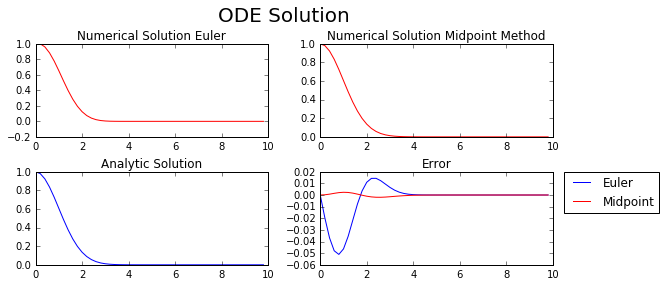
\includegraphics[scale=0.5]{ODE_solution_Euler_Modified}
\caption{Python output: Illustrating upper bound $y^{'}=-xy$ with the initial condition $y(0)=1$ }
\label{Modified Euler Figure}
\end{figure}
for each $i=0,1,...N-1.$

\subsection{2nd Order Runge-Kutta $a_0=0.5$: Heun's method}
\underline{Choosing $a_0=0.5$} gives the unique values $a_1=0.5$, $\alpha_1=h$ and $\beta_1=hf(t,y)$
such that 
\[T^{2}(t,y)=F(t,y) = 0.5 f(t,y)+0.5 f(t+h,y+hf(t,y))-R_1(t+h,y+hf(t,y))
\]
and the error value from
\[ R_1(t+h,y+hf(t,y))=\frac{h^2}{2}\frac{\partial^2 f}{\partial t ^2}(\xi,\mu)
+h^2 \frac{\partial^2 f}{\partial t \partial y}(\xi,\mu)
+\frac{h^2}{2}f(t,y)^2\frac{\partial^2 f}{\partial y^2} (\xi,\mu),
\]for some $\xi \in [t,t+h]$ and $\mu \in [y,y+hf(t,y)]$.\\

Thus Heun's second order Runge-Kutta for the initial value problem
\[y'=f(t,y)\] 
with the initial condition $y(t_0)=\alpha$ is given by
\[w_0=\alpha, \]
\[w_{i+1}=w_i+\frac{h}{2}[f(t_i,w_i)+f(t_i+h,y_i+hf(t_i,w_i))] \]
with an error of order $O(h^2)$.\\
For ease of calculation this can be rewritten as:
\[k_1=f(t_i,w_i),\]
\[k_2=f(t_i+h,w_i+hk_1),\]
\[w_{i+1}=w_i+\frac{h}{2}[k_1+k_2]. \]

\section{Third Order Runge-Kutta methods}
Higher order methods are derived in a similar fashion.
For the Third Order Runge-Kutta methods 
\begin{equation}
\frac{w_{i+1}-w_i}{h}=F(f,t_i,w_i,h),
\end{equation}
with
\begin{equation}
F(f,t,w,h)=a_0k_1+a_1k_2+a_2k_3,
\end{equation}
where 
\[a_0+a_1+a_2=1\] 
and
\[k_1=f(t_i,w_i),\]
\[k_2=f(t_i+\alpha_1h,t_i+\beta_{11}k_1),\]
\[k_3=f(t_i+\alpha_2h,t_i+\beta_{21}k_1+\beta_{22}k_2)).\]
The values of $a_0$, $a_1$, $a_2$, $\alpha_1,\alpha_2$, $\beta_{11}$,$\beta_{21}$, $\beta_{22}$ are derived by group the Taylor expansion,
\begin{eqnarray*} y_{i+1}&=&y_{i}+hf(t_{i},y_{i})+{\frac {h^{2}}{2}}(f_{t}+f_{y}f)_{(t_{i},y_{i})}\\
& &+{\frac {h^{3}}{6}}\left(f_{tt}+2f_{ty}f+f_{t}f_{y}+f_{yy}f^{2}+f_{y}f_{y}f\right)_{(t_{i},y_{i})}\\
& &+O(h^{4}),\end{eqnarray*}
with the 3rd order expand form:
\[ y_{i+1}=y_{i}+ha_{1}f(t_{i},y_{i})+ha_{2}(f+\alpha_{1}hf_{t}+\beta_{11}hf_{y}f\]\[+{\frac {h^{2}}{2}}(f_{tt}\alpha_{1}^{2}+f_{yy}\beta_{11}^{2}f^{2}+2f_{ty}\alpha_{1}\beta_{11}f)+O_{2}(h^{3}))\]
\[+ha_{3}(f+\alpha_{2}hf_{t}+f_{y}\left(\beta_{21}hf+\beta_{22}h(f+\alpha_{1}hf_{t}+\beta_{11}hf_{y}f+O_{3}(h^{2}))\right)\] 
\[+{\frac {1}{2}}(f_{tt}(\alpha_{2}h)^{2}+f_{yy}h^{2}(\beta_{21}f+ \beta_{22}(f+\underbrace {\alpha_{1}hf_{t}+\beta_{11}hf_{y}f+O_{4}(h^{2})}_{O_{5}(h)}))^{2}\]
 \[+2f_{ty}\alpha_{2}h^{2}(\beta_{21}f+\beta_{22}(f+\underbrace {\alpha_{1}hf_{t}+\beta_{11}hf_{y}f+O_{4}(h^{2})}_{O_{5}(h)})))).\]
 This results in 8 equations with 8 unknowns, but only 6 of these equations are independent. For this reason the are two free parameters to choose.

For example, we can choose that \[\alpha_{2}=1,\beta_{11}=\frac{1}{2},\]then we obtain the following difference equation.
\[ w_{i+1}=w_{i}+{\frac {h}{6}}(k_{1}+4k_{2}+k_{3}),\]
where
\[k_{1}=f(t_{i},w_{i}),\]
\[ k_{2}=f(t_{n}+1/2h,w_{n}+1/2hk_{1}),\]
\[ k_{3}=f(t_{n}+h,w_{n}-hk_{1}+2hk_{2}).\]

\section{Runge-Kutta fourth order}
The most commonly used Runge-Kutta method is the 4th Order Runge-Kutta method, which is given by the formulae,
\[w_0 = \alpha, \]
\[k_1 = hf(t_i,w_i), \]
\[k_2 = hf(t_i+\frac{h}{2},w_i+\frac{1}{2}k_1), \]
\[k_3 = hf(t_i+\frac{h}{2},w_i+\frac{1}{2}k_2), \]
\[k_4 = hf(t_{i+1},w_i+k_3), \]
\[w_{i+1}=w_{i}+\frac{1}{6}(k_1+2k_2+2k_3+k_4). \]
\begin{example}
Example Midpoint method,
\[y^{'}=y-t^2+1, \ \ \ 0 \leq t \leq 2, \ \ \ y(0)=0.5, \]
\[N=10, \ \ \ t_i=0.2i, \ \ \ h=0.2, \]
\[w_0=0.5, \]
\begin{eqnarray*}
w_{i+1} &=& w_{i} + 0.2f(t_i+\frac{0.2}{2},w_i+\frac{0.2}{2}f(t_i,w_i))\\
 &=& w_{i} + 0.2f(t_i+0.1,w_i+0.1(w_i-t^2_i+1))\\
 &=& w_{i} + 0.2(w_i+0.1(w_i-t^2_i+1)-(t_i+0.1)^2+1)\\
\end{eqnarray*}
\end{example}

\begin{example}
Example Runge-Kutta fourth order method
\[y^{'}=y-t^2+1, \ \ \ 0 \leq t \leq 2, \ \ \ y(0)=0.5, \]
\[N=10, \ \ \ t_i=0.2i, \ \ \ h=0.2, \]
\[w_0=0.5, \]
\begin{eqnarray*}
k_1&=&h(w_i-t_i^2+1),\\
k_2&=&h(w_i+\frac{1}{2}k_1-(t_i+\frac{h}{2})^2+1)\\
k_3&=&h(w_i+\frac{1}{2}k_2-(t_i+\frac{h}{2})^2+1)\\
k_4&=&h(w_i+\frac{1}{2}k_3-(t_i+h)^2+1)\\
w_{i+1} &=& w_{i} + \frac{1}{6}(k_1+2k_2+2k_3+k_4)
\end{eqnarray*}
\begin{figure}[H]
\centering
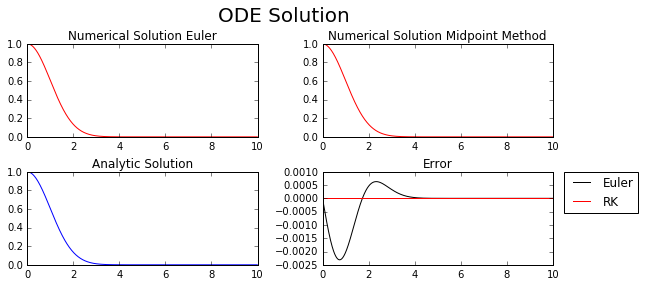
\includegraphics[scale=0.5]{ODE_solution_Euler_RK}
\caption{Python output: Illustrating upper bound $y^{'}=-xy$ with the initial condition $y(0)=1$ }
\label{RK vs Euler Figure}
\end{figure}
\begin{figure}[H]
\centering
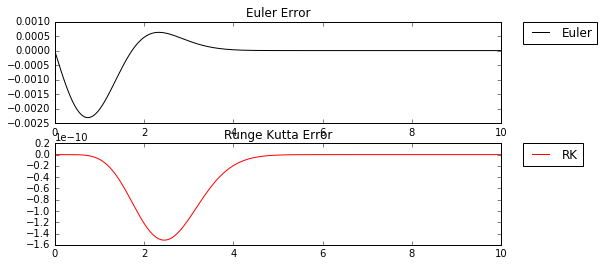
\includegraphics[scale=0.5]{ODE_error_RK_Euler}
\caption{Python output: Illustrating upper bound $y^{'}=-xy$ with the initial condition $y(0)=1$ }
\label{Modified Euler Figure}
\end{figure}
\end{example}
\section{Butcher Tableau}

Another way of representing a Runge-Kutta method is called the Butcher tableau named after John C Butcher (31 March 1933).

\[ y_{i+1}=y_{i}+h\sum_{n=1}^{s}a_{n}k_{n},\] 
where

\[ {\begin{aligned}k_{1}&=f(t_{i},y_{i}),\\k_{2}&=f(t_{i}+\alpha_{2}h,y_{i}+h(\beta_{21}k_{1})),\\k_{3}&=f(t_{i}+\alpha_{3}h,y_{i}+h(\beta_{31}k_{1}+\beta_{32}k_{2})),\\&\ \ \vdots \\k_{s}&=f(t_{i}+\alpha_{s}h,y_{i}+h(\beta_{s1}k_{1}+\beta_{s2}k_{2}+\cdots +\beta_{s,s-1}k_{s-1})).\end{aligned}}\] 

These data are usually arranged in a mnemonic device, known as a Butcher tableau
\begin{center}
 \begin{tabular}{c| c c c c c} 
 0&  &  & & & \\ 
 $\alpha_2$& $\beta_{21}$ &  & & & \\ 
 $\alpha_3$& $\beta_{31}$ & $\beta_{31}$ & & & \\ 
 $\vdots $& $\vdots$ & $\vdots$  & & & \\ 
 
 $\alpha_s$& $\beta_{s1}$ & $\beta_{s2}$ & $\cdots$& $\beta_{ss-1}$ & \\ 
 \hline
 & $a_{1}$  & $a_{2}$ & $\cdots$ &$a_{s-1}$ & $a_s$ \\ 
\end{tabular}
\end{center}
The method is consistent if 
\[\sum_{j}^{s-1} \beta_{sj}=\alpha_s.\]
\subsection{Heun's Method}
The Butcher's Tableau for Heun's Method is:
\begin{center}
 \begin{tabular}{c| c c} 
 $0$&    &   \\ 
 $1$& $1$ &   \\ 
 \hline
 & $\frac{1}{2}$  & $\frac{1}{2}$   \\ 
\end{tabular}
\end{center}
\subsection{4th Order Runge-Kutta}
The Butcher's Tableau for the 4th Order Runge-Kutta is:
\begin{center}
 \begin{tabular}{c| c c c c} 
 $0$&    &  & & \\ 
 $\frac{1}{2}$& $\frac{1}{2}$ &  & & \\ 
 $\frac{1}{2}$& $0$ & $\frac{1}{2}$ & &  \\ 
 $1 $& $0$ & $0$  &$1$ &  \\ 
 \hline
 & $\frac{1}{6}$  & $\frac{2}{6}$ & $\frac{2}{6}$ &$\frac{1}{6}$  \\ 
\end{tabular}
\end{center}

\section{Convergence Analysis}
In order to obtain convergence of the general Runge-Kutta we need to have the truncation
$\tau_n(y)\rightarrow0$ as $h \rightarrow 0$.  Since,
\[\tau(y)=\frac{y(t_{n+1})-y(t_n)}{h}-F(t_n,y(t_n),h;f), \]
we require,
\[F(x,y,h;f)\rightarrow y{'}(x)=f(x,y(x)). \]
More precisely define,
\[\delta(h)= \max_{a\leq t \leq b ; -\infty < y <\infty} |f(t,y)-F(t,y,h;f)|, \]
and assume,
\begin{equation}
\label{C}
 \delta(h) \rightarrow 0, \ \ \ \mbox{ as } h \rightarrow 0.
 \end{equation}
This is called the \underline{consistency condition} for the RK method.\\
We will also need a \addtoindex{Lipschitz Condition} on $F$:
\begin{equation}
\label{L}
|F(t,y,h;f)-F(t,z,h;f)|\leq |y-z|,
 \end{equation}
for all $a\leq t \leq b$ and $-\infty <y,z < \infty $ and small $h >0$.
\begin{example}
Looking at the midpoint method
\begin{eqnarray*}
|F(t,w,h;f)-F(t,z,h;f)| &=&
\left|f(t+\frac{h}{2},w+\frac{h}{2}f(t,w)) \right. \\
& & \left. -f(t+\frac{h}{2},z+\frac{h}{2}f(t,z) )
 \right|\\
&\leq& K \left| w-z +\frac{h}{2}[f(t,w)-f(t,z) ]\right|\\
&\leq &	K \left(1 +\frac{h}{2}K \right)|w-z|
\end{eqnarray*}
\end{example}
\begin{theorem}
Assume that the Runge-Kutta method satisfies the \addtoindex{Lipschitz Condition}. Then
for the initial value problems
\[ y^{'}=f(x,y),\]
\[ y(x_0)=y_0. \]
The numerical solution $\{ w_n\}$ satisfies
\[ \max_{a\leq x\leq b}|y(x_n)-w_n| \leq e^{(b-a)L}|y_0-w_0|+\left[\frac{e^{(b-a)L}-1}{L} \right]\tau(h) \]
where
\[\tau(h) = \max_{a\leq x\leq b}|\tau_n(h)|,\]
If the consistency condition 
\[ \delta(h) \rightarrow 0 \mbox{ as  } h\rightarrow 0, \]
where
\[\delta(h) = \max_{a \leq x \leq b}|f(x,y)-F(x,y;h;f)|. \]

\end{theorem}
\begin{proof}
Subtracting
\[ w_{n+1}=w_n +hF(t_n,w_n,h;f),\]
and
\[y( t_{n+1})=y(t_n) +hF(t_n,y(t_n),h;f)+h\tau_n(h),\]
we obtain
\[ e_{n+1}=e_n +h[F(t_n,w_n,h;f)-F(t_n,w_n,h;f)]+h\tau_n(h),\]
in which $e_n=y(t_n)-w_n$. Apply the \addtoindex{Lipschitz Condition} $L$ and the truncation
error we obtain
\[|e_{n+1}| \leq (1+hL)|e_n| + h \tau_n(h). \]
This nicely leads to the result.\\
In most cases it is known by direct computation that $\tau(h) \rightarrow 0$ as $h \rightarrow 0$
an in that case convergence of $\{w_n \}$ and $y(t_n)$ is immediately proved.
\\
But all we need to know is that (\ref{C}) is satisfied .  To see this we write
\[\begin{array}{ccc}
h\tau_n &=& y( t_{n+1})-y(t_n) -hF(t_n,y(t_n),h;f),\\
&=&hy^{'}(t_n)+\frac{h^{2}}{2}y^{''}(\xi_n) -hF(t_n,y(t_n),h;f),\\
h|\tau_n| &\leq& h\delta(h)+\frac{h^{2}}{2}|y^{''}|.\\
|\tau_n| &\leq& \delta(h)+\frac{h}{2}|y^{''}|.\\
\end{array}
\]
Thus $\tau(h) \rightarrow 0$ as $h \rightarrow 0$
\end{proof}
From this we have
\begin{corollary}
If the RK method has a truncation error $\tau(h)=O(h^{m+1})$ then the rate of
convergence of $\{w_n\}$ to $Y(t)$ is $O(h^m)$.
\end{corollary}

\section{The choice of method and step-size}
An interesting question is since \addtoindex{Runge-Kutta method} is 4th order but requires 4 steps and Euler
only required 3 is it more beneficial to use a smaller h than a higher order method?\\
But this does lead us to the question of how do we define our h to maximize
the solution we have.\\
An ideal difference-equation method
\[w_{i+1}=w_i+h\phi(t_i,w_i,h) \ \ \ i=0,..,n-1 \]
for approximating the solution $y(t)$ to the \addtoindex{Initial Value Problem}
$ y^{'} = f(t,y)$ would have the property that given a tolerance $\varepsilon >0$
the minimal number of mesh points would be used to ensure that the global error
$|y(t_i)-w_i|$ would not exceed $\va$ for any $i=0,...,N.$\\
We do this by finding an appropriate choice of mesh points. Although we cannot 
generally determine the global error of a method there is a close relation between 
local truncation and global error.  By using methods of differing order we can predict the local truncation error and using this prediction choose a step size
that will keep global error in check.\\
Suppose we have two techniques
\begin{enumerate}
\item
An nth order Taylor method of the form
\[y(t_{i+1}) = y(t_i) +h\phi(t_i,y(t_i),h_i)+O(h^{n+1}) \]
producing approximations
\[w_0=\alpha \]
\[w_{i+1}=w_i +h\phi(t_i,w_i,h_i)\]
with local truncation $\tau_{i+1}=O(h^n).$
\item
An (n+1)st order Taylor of the form
\[y(t_{i+1}) = y(t_i) +h\psi(t_i,y(t_i),h_i)+O(h^{n+2}) \]
producing approximations
\[v_0=\alpha \]
\[v_{i+1}=v_i +h\psi(t_i,v_i,h_i)\]
with local truncation $\upsilon_{i+1}=O(h^{n+1}).$
\end{enumerate}
We first make the assumption that $w_i \approx y(t_i) \approx v_i$ and choose a fixed
step size to generate $w_{i+1}$ and $v_{i+1}$ to approximate $y(t_{i+1})$.  Then
\begin{eqnarray*}
\tau_{i+1} & = & \frac{y(t_{i+1})-y(t_i)}{h} - \phi(t_i,y(t_i),h) \\
& = &  \frac{y(t_{i+1})-w_i}{h} - \phi(t_i,w_i,h) \\
& = &  \frac{y(t_{i+1})-(w_i+h\phi(t_i,w_i,h))}{h} \\
& = &  \frac{y(t_{i+1})-w_{i+1}}{h} 
\end{eqnarray*}
Similarly
\[ \Upsilon_{i+1} =\frac{y(t_{i+1})-v_{i+1}}{h} \]
As a consequence
\begin{eqnarray*}
\tau_{i+1} &=& \frac{y(t_{i+1})-w_{i+1}}{h} \\
 &=& \frac{(y(t_{i+1})-v_{i+1})+(v_{i+1}-w_{i+1})}{h} \\
 &=& \Upsilon_{i+1}(h)+\frac{(v_{i+1}-w_{i+1})}{h}. 
\end{eqnarray*}
but $\tau_{i+1}(h)$ is $O(h^n)$ and $\Upsilon_{i+1}(h)$ is $O(h^{n+1})$ so the 
significant factor of $\tau_{i+1}(h)$ must come from $\frac{(v_{i+1}-w_{i+1})}{h}$.  This gives us an easily computed approximation of $O(h^n)$ method,
\[\tau_{i+1} \approx \frac{(v_{i+1}-w_{i+1})}{h}.  \]
The object is not to estimate the local truncation error but to adjust step size to 
keep it within a specified bound.  To do this we assume that since $\tau_{i+1}(h)$ is $O(h^n)$ a number $K$ independent of $h$ exists with, \[\tau_{i+1}(h) \approx Kh^n. \]
Then the local truncation error produced by applying the nth order method with a
new step size $qh$ can be estimated using the original approximations $w_{i+1}$ 
and $v_{i+1}$
\[\tau_{i+1}(qh) \approx K(qh)^n \approx q^n\tau_{i+1}(h) \approx \frac{q^n}{h}(v_{i+1}-w_{i+1}), \]
to bound $\tau_{i+1}(qh)$ by $\va$ we choose $q$ such that
\[\frac{q^n}{h}|v_{i+1}-w_{i+1}|\approx \tau_{i+1}(qh) \leq \va, \]
which leads to
\[ q \leq \left( \frac{\va h }{|v_{i+1}-w_{i+1}|}\right)^{\frac{1}{n}}, \]
which can be used to control the error.


\newpage
\section{Problem Sheet 3 - Runge-Kutta}
\begin{enumerate}


\item
Apply the Midpoint Method to approximate the solution of the given initial value problems using the indicated number of time steps. Compare the approximate solution with the given exact solution
\begin{enumerate}
\item
$y'=t-y, \ \ (0\leq t \leq 4),$\\
with the initial condition $y(0)=1,$\\
$N=4$, 
with the exact solution
$y(t)=2e^{-t}+t-1.$\\

\item 
$y'=y-t, \ \ (0\leq t \leq 2),$\\
with the initial condition $y(0)=2,$\\
$N=4$, 
with the exact solution
$y(t)=e^{t}+t+1.$\\

\end{enumerate}
\item
Apply the 4th Order Runge-Kutta Method to approximate the solution of the given initial value problems using the indicated number of time steps. Compare the approximate solution with the given exact solution
\begin{enumerate}
\item
$y'=t-y, \ \ (0\leq t \leq 4),$\\
with the initial condition $y(0)=1,$\\
$N=4$, 
with the exact solution
$y(t)=2e^{-t}+t-1.$\\

\item 
$y'=y-t, \ \ (0\leq t \leq 2)$\\
with the initial condition $y(0)=2,$\\
$N=4$, with the exact solution
$y(t)=e^{t}+t+1.$\\

\end{enumerate}
\item
Derive the difference equation for the Midpoint Runge-Kutta method\\
\[ w_{n+1}=w_n+k_2,\]
\[k_1=hf(t_n,w_n),\]
\[k_2=hf(t_n+\frac{1}{2}h,w_n+\frac{1}{2}k_1)\]
for solving the ordinary differential equation
\[ \frac{dy}{dt}=f(t,y), \]
\[y(t_0)=y_0, \]
by using a formula of the form
\[w_{n+1}=w_n+ak_1+bk_2, \]
where $k_1$ is defined as above,
\[k_2=hf(t_n+\alpha h,w_n+\beta k_1),\]
and $a$, $b$, $\alpha$ and $\beta$ are constants are determined. Prove that $a+b=1$ and $b\alpha=b\beta=\frac{1}{2}$ and choose appropriate values to give the Midpoint Runge-Kutta method.


\end{enumerate}
\newpage